
\chapter{Ferramenta desenvolvida}
\label{cap:metodologia}
% O resultado obtido é a ferramenta 

% Detalhes da execução (linhas de código, prints, etc...), o que está sendo escaneado em produção

\section{Módulos Implementados}

    \begin{figure}[H]
        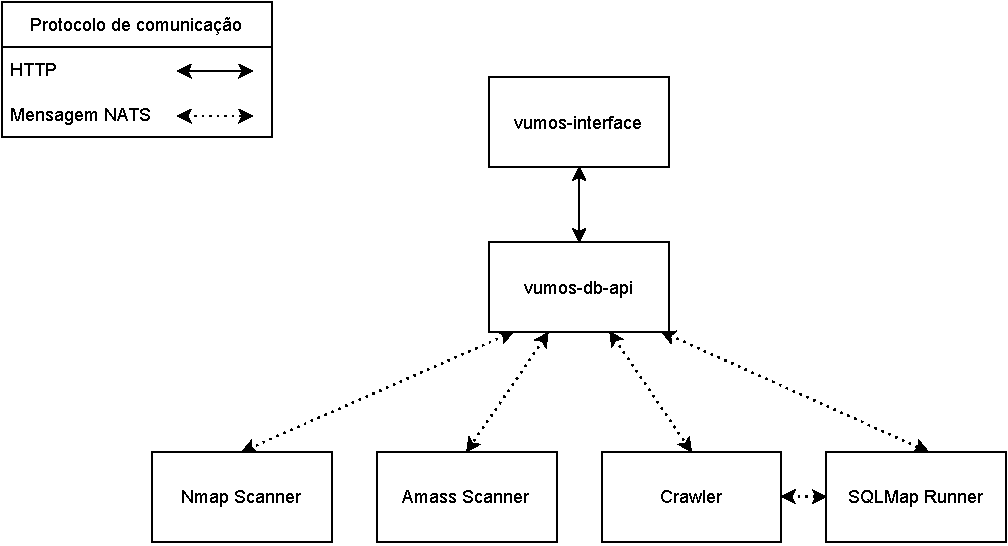
\includegraphics[scale=0.8]{figuras/vumos-Microservices.pdf}
        \caption{Diagrama de comunicação dos microsserviços implementados.\label{fig:microservices}}
    \end{figure}

    \subsection{Vumos Common}
    Seguindo a arquitetura de microsserviços, cada módulo é responsável pelo armazenamento das informações relevantes a seu funcionamento, podendo ser elas obtidas através do prório módulo ou através de mensagens recebidas por outros módulos. 
    
    Para facilitar o processo de desenvolvimento de um novo módulo, foi implementada uma biblioteca em \textit{Python} que funciona como arcabouço para os outros módulos, e também contém o \textit{schema} das mensagens da aplicação.
    
    Ele conta com um banco de dados local implementado em SQLite, usado principalmente para o armazenamento das configurações do módulo. Para facilitar o seu acesso do ponto de vista do desenvolvedor, foi implementado um conjunto de funções que tornam o seu uso transparente.
    
    Para que seja possível enviar e receber mensagens do módulo enquanto ele executa outras tarefas, como escrita no banco de dados ou requisições HTTP, foi utilizada uma arquitetura de computação assíncrona, utilizando a biblioteca \textit{asyncio} do Python. Isso nos proporciona métodos interessantes para a execução de subprocessos, o que é necessário para uma grande parte dos módulos a serem implementados, além de proporcionar um maior desempenho no que se diz respeito a esse tipo de operação. 

    \subsection{Amass Scanner}
    
    Este módulo tem como objetivo encontrar subdomínios existentes no domínio principal \url{usp.br}, usando para isso a ferramenta de código aberto AMASS \footnote{\url{https://github.com/OWASP/Amass}}. Esta ferramenta utiliza diversas técnicas de enumeração de DNS para tentar encontrar subdomínios válidos, como a força bruta, \textit{search engine scraping}, busca em certificados e páginas arquivadas.
    
    Como variáveis configuráveis deste módulo, temos somente:
    \begin{itemize}
    \item \emph{Initial Domain}: Domínio inicial que será escaneado recursivamente
    \end{itemize}
    
    Uma vez encontrados os subdomínios, é enviada uma mensagem como \textit{broadcast} com os tal informação em seus respectivos hosts/alvos.
    % TODO: link com vumos-db-api falando dos targets?
    \subsection{Nmap Scanner}
    Este módulo tem como objetivo encontrar máquinas na rede e seus serviços, obtendo também informações sobre eles, como em quais portas estão rodando, quais versões, e possivelmente se possuem alguma vulnerabilidade conhecida. Para isso, é utilizada a ferramenta de código aberto de mapeamento de rede NMAP \footnote{\url{https://github.com/nmap/nmap}}, que realiza todas essas funções para cada um dos IPs que ela encontra.
    
    Como variáveis configuráveis deste módulo, temos:
    \begin{itemize}
        \item \emph{Flags}: São os argumentos de linha de comando que serão enviados ao NMAP, ativando ou desativando cada uma de suas features. Por exemplo, aqui podemos ativar ou desativar a busca automatizada por vulnerabilidades conhecidas.
        \item \emph{Redo Days}: Quantidade de dias até que o escaneamento seja realizado novamente
        \item \emph{IP Ranges}: Quais IPs serão escaneados. São aceitos IPs no formato \textit{CIDR Standard} separados por vírgula, ou seja, é possível definí-lo para escanear todas as subredes da USP de uma vez.
    \end{itemize}
    
    Por fim, para cada serviço encontrado é enviada uma mensagem como \textit{broadcast} e também é enviada uma mensagem com seu alvo.
    
    \subsection{Crawler}
    Este módulo tem o objetivo de, a partir de uma página HTML inicial, encontrar novas páginas que possuem links dinâmicos. Isso é feito usando um \textit{crawler} customizado que utiliza o módulo de Python Scrapy \footnote{\url{https://scrapy.org/}}. Como não é possível saber se um link é processado dinamicamente ou não pelo servidor sem uma análise extensa em cada um deles, é utilizada uma heurística, que nos permite conseguir uma grande quantidade de links dinâmicos sem processamento extra. Portanto, uma URL é considerada dinâmica se contiver uma interrogação (indicando que contém parâmetros, sendo eles analisados para uso futuro), ou se for o resultado de um envio de formulário, onde os parâmetros são seus campos. 
    
    Como variáveis configuráveis deste módulo, temos:
    \begin{itemize}
        \item \emph{Allowed domains}: Domínios onde o crawler é permitido a rodar. Isso impede que domínios fora do escopo sejam escaneados quando um link externo (como do Youtube, por exemplo) for encontrado.
        \item \emph{Initial URLs}: Lista separada por vírgulas com as URLs por onde o crawler começará a procurar links. 
    \end{itemize}
    
    Para cada URL dinâmica encontrada, é enviada uma mensagem como \textit{broadcast} e também é enviada uma mensagem com seu alvo e com seu serviço, sendo tais informações extraidas tanto da URL em si quanto da página que a contém.
    
    \subsection{SQLMap Runner}
    Este módulo tem como objetivo procurar vulnerabilidades de SQL Injetion em uma determinada URL dinâmica através da ferramenta de código aberto SQLMap \footnote{\url{https://github.com/sqlmapproject/sqlmap}}. Para isso, este módulo escuta pelas mensagens de \textit{broadcast} do tipo \textit{Path}, que são enviadas pelo módulo do Crawler e, para cada uma delas, coloca numa fila persistente em disco. Isso é feito pois o SQLMap, devido à sua complexidade, demora diversas vezes mais para ser executado em relação ao Crawler, portanto as URLs são acumuladas nesta fila e processadas assim que possível.
    
    Para tornar o processo mais rápido, este módulo implementa também um sistema de \textit{multithreading}, no qual diversas instâncias do SQLMap são executadas ao mesmo tempo em URLs diferentes para paralelizar o processo. Para tal, foi utilizado o gerenciamento de \textit{threads} de execução do \textit{asyncio}, onde cada instância do SQLMap é iniciado em uma co-rotina assíncrona com um executor próprio.
    
    Para buscar tais vulnerabilidades, o SQLMap executa diversas requisições HTTP com alterações em seus parâmetros, e verifica por diferenças nos resultados, de acordo com as seguintes técnicas:
    
    \label{item:sqlmap}
    \begin{itemize}
        \item \emph{Boolean-based blind}: Em português "ataque cego baseado em booleanos", esta técnica adiciona parâmetros de SQL na requisição HTTP que retornem ou verdadeiro ou falso, e verifica a página de resposta por diferenças entre os dois valores. Dessa forma, esta técnica é capaz de extrair dados caractere a caractere, utilizando o método da bisseção para diminuir a quantidade de requisições necessárias para as comparações.
        
        \item \emph{Time-based blind}: Em português "ataque cego baseado em tempo", esta técnica funciona de forma similar a anterior, porém é capaz de extrair dados até mesmo quando a aplicação não retorna valores diferentes para verdadeiro e falso em sua página de resposta. Isso é feito através da inserção de um comando \textit{SLEEP}, que faz a aplicação demorar mais para responder em caso positivo. Em seguida, é medido o tempo de resposta de cada requisição, e com isso é possível inferir se o resutado foi positivo ou negativo, e é aplicado o método da biseção novamente.
        
        \item \emph{Error-based}: Em português "ataque baseado em erros", esta técnica só funciona quando a aplicação retorna o erro do sistema gerenciador de banco de dados (SGBD) para o usuário. Ela envia uma requisição que contém um comando que provoque um erro no SGBD após a execução da query de extração de dados, dessa forma os resultados são exibidos na página de erro e podem ser facilmente extraídos.
        
        \item \emph{UNION query-based}: Em português "ataque baseado em requisições UNION", esta técnica adiciona envia requisições SQL que contém um UNION, de forma que quando os resultados da aplicação forem exibidos, os valores que desejam ser extraídos também estarão presentes. 
        
        \item \emph{Stacked Queries}: Em português "requisições empilhadas", esta técnica é mais focada na inserção de dados e execução de comandos arbitrários no SGBD. Ela verifica se a aplicação suporta multiplas requisições SQL por requisição HTTP com o uso de um ";", e em caso positivo, é possível executar qualquer tipo de comando SQL sem restrição da aplicação HTTP.
    \end{itemize}
    
    Como variáveis configuráveis deste módulo, temos:
    \begin{itemize}
        \item \emph{Number of instances}: Quantidade de instâncias do SQLMap que serão executadas ao mesmo tempo.
        \item \emph{SQLMap Techniques}: Cadeia de caracteres que representa quais técnicas de injeção serão testadas em cada um dos sites.
        \item \emph{SQLMap Level}: Número inteiro de 1 a 5 que representa o nível de execução do SQLMap. Tal valor representa o quão minucioso o SQLMap será em sua busca por vulnerabilidades, sendo um nível maior mais exaustivo, mas também mais demorado.
    \end{itemize}
    
    Uma vez encontrada uma página vulnerável, é enviada uma mensagem como \textit{broadcast} anunciando-a, com todas as informações pertinentes.


    \subsection{vumos-db-api}
    
    Este é o módulo central da aplicação, que é responsável por controlar os outros módulos e receber seus dados para armazenamento e exibição ao usuário. Ao contrário dos módulos acima, ele foi feito usando NodeJS, Express e Typescript , e utiliza um banco de dados PostgreSQL, que permite o uso de algumas de suas funcionalidades mais avançadas pela biblioteca de ORM (Object-Relational Mapping, ou Mapeamento Objeto-Relacional) TypeORM. 
    
        % TODO: falar do DB, postgres e mostrar um diagrama
    \subsection{vumos-interface}
        % TODO: botar uns prints bonitinhos
    

\section{Orquestração}
    
    % TODO: falar das networks 

\section{Produção}
    O VuMoS foi colocado em produção em http://vumos.hackersdobem.sti.usp.br/ e já está atualmente escanenado todos os subdomínios de \url{usp.br} e também todas as subredes da universidade. 

% TODO: falar da organização dos repositórios
